Four cavities were modelled, using coupled wave theory and exact theory, during this project. Firstly a simple cavity reproducing the results proposed by Topf and McCall\cite{topf_modes_2014}, secondly a chiral cavity with a defect introduced at the centre of the cavity, then, a hybrid cavity composed of a right-handed medium placed between two left-handed media, and finally, a hybrid cavity similar to the previous one, except it has a defect in the centre. This chapter aims to describe the method used to ensure the correctness and a good understanding of the processes that are taking place inside the cavities.

\section{Reflectivity}

The first step to ensure the correctness of the simulation is to reproduce the reflectivity diagram presented in previous studies\cite{mccall_simplified_2009}. As the source code used to calculate those reflectivity diagrams is available, a direct comparison with the coupled wave and exact theories implementations used for this report is possible. The reflectivity of the cavity with a defect is also plotted for both simulation methods, as it is expected to give a very narrow filter because of the similarity with a quarter wavelength defect in a standard distributed Bragg reflector\cite{mccall_photonics_2020}. The reflectivity diagram for the third cavity was not examined.

\section{Energy conservation}

To check the correctness of the models used, it is worth checking the energy conservation throughout a lossless medium. To compare coupled wave theory to exact theory, equations \ref{eq:energyconservationa}, \ref{eq:energyconservationb} and \ref{eq:energyconservationredistribution} are plotted for the each cavity, with the gain turned to zero.

\section{Conditions for lasing}
This section discusses the method used to detect cavity susceptible to allow lasing. Two equivalent conditions are presented, as well as the parameters examined.

\subsection{First lasing condition}
In order to characterize the round-trip of a ray in the cavity, we consider the field at $z=0^-$. The chiral medium is characterized by the matrix $\bm{M_c}$. Applying equation \ref{eq:pinv} yields equation \ref{eq:method:internal_pinv}.

\begin{equation}
\begin{bmatrix}
E_{L}^+(z=L^-) \\
E_{R}^+(z=L^-) \\
E_{L}^-(z=0^+) \\
E_{R}^-(z=0^+) \\
\end{bmatrix} = \left(\text{inv}_1(\bm{M_c})\right)^{-1}\begin{bmatrix}
E_{L}^+(z=0^+) \\
E_{R}^+(z=0^+) \\
E_{L}^-(z=L^-) \\
E_{R}^-(z=L^-) \\
\end{bmatrix}\label{eq:method:internal_pinv}
\end{equation}
Then, using equation \ref{eq:reflection}, it is possible to express the boundary condition at the interfaces with the isotropic media. Naming $\bm{R_1}$ and $\bm{R_2}$ the reflection matrices at interfaces 1 and 2, this yields equation \ref{eq:method:round_trip}, where $F_0$ and $F_1$ are the field vectors before and after a round trip.
\begin{equation}
F_1 = \begin{pmatrix}
\bm{0} & \bm{R_1}\\
\bm{R_2} & \bm{0}
\end{pmatrix}\left(\text{inv}_1(\bm{M_c})\right)^{-1}F_0 \label{eq:method:round_trip}
\end{equation}
Then it is straightforward to express the lasing condition as in equation \ref{eq:method:round_trip_det}, where $\bm{I}$ is the identity matrix.
\begin{equation}
\left|\begin{pmatrix}
\bm{0} & \bm{R_1}\\
\bm{R_2} & \bm{0}
\end{pmatrix}\left(\text{inv}_1(\bm{M_c})\right)^{-1} - \bm{I}\right| = 0 \label{eq:method:round_trip_det}
\end{equation}

\subsection{Second lasing condition}
\label{sec:lasing_condition}
This second method is simpler than the first and will be used to analyze the cavities. Its key advantage is that it allows using the propagation matrix describing the cavity as a "black box", that is, it is not necessary to be able to express the reflections at the interfaces. This allows simulating the cavities using the Oseen transformation.

Considering a cavity described by the propagation matrix $\bm{M_c}$, we have equation \ref{eq:method:propag}.

\begin{equation}
\begin{bmatrix}
E_{L}^+(z=L^+) \\
E_{R}^+(z=L^+) \\
E_{L}^-(z=L^+) \\
E_{R}^-(z=L^+) \\
\end{bmatrix} = \bm{M_c}\begin{bmatrix}
E_{L}^+(z=0^-) \\
E_{R}^+(z=0^-) \\
E_{L}^-(z=0^-) \\
E_{R}^-(z=0^-) \\
\end{bmatrix}\label{eq:method:propag}
\end{equation}
%
For a laser cavity, the boundary conditions are $E_{L}^-(z=L^+)=0,\;E_{R}^-(z=L^+)=0$ and $E_{L}^+(z=0^-)=0,\;E_{R}^+(z=0^-)=0$. Thus, writing $\bm{M_c}$ by $2\times2$ blocks, equation \ref{eq:method:propag} becomes
\begin{equation}
\begin{bmatrix}
E_{L}^+(z=L^+) \\
E_{R}^+(z=L^+) \\
0 \\
0 \\
\end{bmatrix} = \begin{pmatrix}
	\bm{M_{11}} & \bm{M_{12}}\\
	\bm{M_{21}} & \bm{M_{22}}
\end{pmatrix}\begin{bmatrix}
0 \\
0 \\
E_{L}^-(z=0^-) \\
E_{R}^-(z=0^-) \\
\end{bmatrix}
\end{equation}
%
Then a simple condition for lasing can be expressed by equation \ref{eq:method:lasing_condition}.
\begin{equation}
\left|\bm{M_{22}}\right| = 0 \label{eq:method:lasing_condition}
\end{equation}

\subsection{Parameters of the simulations}

The parameters explored in this study are gain and detuning of the medium. Those two quantities are defined from $\delta k$, introduced in section \ref{sec:cwt}, and $L$ the length of the medium considered. Denoting gain and detuning respectively $g$ and $d$,
\begin{eqnarray}
	g &=& - \Im{\frac{\delta k}{2}L}\\
	d &=& \Re{\frac{\delta k}{2}L}
\end{eqnarray}
%
The coupling $\kappa$ for all the chiral media is fixed to $\kappa=4/L$, and the periodicity of the medium, $L_p$, is fixed to 300nm.

These parameters cannot be used directly with Oseen transformation. However $k$, the wave-vector in the medium, and thus $\bar{n}$ can be determined directly from $\delta k$, allowing to calculate the permittivities $\epsilon_{a,b}$ as follow.
\begin{eqnarray}
\epsilon_a &=& \bar{n}^2 + \frac{2\kappa\bar{n}}{k_0}\\
\epsilon_b &=& \bar{n}^2 - \frac{2\kappa\bar{n}}{k_0}
\end{eqnarray} 

To provide better visualisation of lasing modes, as well as enable their automatic detection, the modelisations described in this report use the logarithm of the invert of equation \ref{eq:method:lasing_condition}. Thus, favourable lasing conditions can be identified as sharp peaks on the plots.



\section{Output polarization and intensity distribution of the modes}
\label{sec:output_pol}
It is then possible characterize the modes outputted by the cavity. Indeed, once the lasing cavities have been identified using method described in section \ref{sec:lasing_condition}, the corresponding output mode is found by taking the eigenvector of $\bm{M_{22}}$ with a 0 eigenvalue\footnote{In the simulations, the eigenvector with the smallest absolute eigenvalue is chosen.}.
\subsection{Comparison of the output polarisation ellipse}

The field is expressed in the cartesian or electromagnetic basis\footnote{In the case of a laser cavity, since there is not field coming towards the cavity, $E_{x,y}^-(z<0)=E_{x,y}(z<0)$}. Then, defining $R$ and $\delta$ as in equation \ref{eq:method:Rdelta},
\begin{equation}
R = \atan(|E_x|+|E_y|),\;\delta = \arg(E_y) - \arg(E_x) \label{eq:method:Rdelta}
\end{equation}
it is possible to calculate angle $\epsilon$ and orientation $\theta$ of the ellipse as in equations \ref{eq:method:epsilon} and \ref{eq:method:theta}\cite{weir_optical_2019}.
\begin{eqnarray}
\epsilon &=& \frac{1}{2}\asin(\sin(2R)|\sin(\delta)|) \label{eq:method:epsilon}\\
\theta &=& \frac{1}{2}\atan(\tan(2R)\cos(\delta)) \label{eq:method:theta}
\end{eqnarray}
$\epsilon$ and $\theta$ relate to the output polarization ellipse as in figure \ref{fig:ellipse}. The handedness of the ellipse can be determined from the sign of $\delta$, but since all calculations in this study are carried in the circular basis, it is simpler to look at the amplitude of $E_L$ and $E_R$. The polarizations outputted by the cavities is compared \textit{via} their corresponding values of $\epsilon$ and $\theta$, as well as the handedness of the ellipse.

In order to draw the ellipse, the cartesian form is used, and then rotated by angle $\theta$. The semi-major and semi-minor axes, $a$ and $b$, relate to $\epsilon$ as in equation \ref{eq:tanepsilon}. Thus, $\epsilon$ gives a good measure of how close to a circular polarisation the output is, as a circle would present $\epsilon=45^\circ$.
\begin{equation}
\frac{b}{a}=\tan(\epsilon) \label{eq:tanepsilon}
\end{equation}
%
Then, the points of the ellipse, before rotation, verify equation \ref{eq:epsilon}.
\begin{equation}
R^2 = ax^2+by^2\label{eq:ellipse}
\end{equation}


\begin{figure}
	\centering
	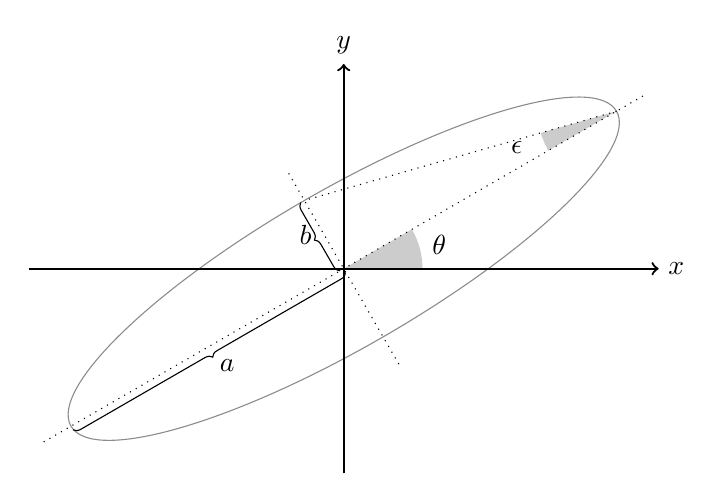
\begin{tikzpicture}[scale=2]
		\fill[color=gray!40] (0.5,0) arc (0:30:0.5) -- (0,0) -- (0.5,0);
		\draw (0.5,0.15) node[right] {$\theta$};
		\begin{scope}[rotate=30]
			\fill[color=gray!40] (1.5,0) arc (-180:-194:0.5) -- (2,0) -- cycle;
			\draw[color=gray!90] (0,0) ellipse (2 and 0.5);
			\draw[dotted] (-2.2,0) -- (2.2,0);
			\draw[dotted] (0,-0.7) -- (0,0.7);
			\draw[dotted] (2,0) -- (0,0.5);
			\draw (1.3,0.25) node[below right] {$\epsilon$};
			\draw[decoration={brace,mirror,raise=1.5pt},decorate]
			(0,0.5) -- node[left=1pt] {$b$} (0,0);
			\draw[decoration={brace,mirror,raise=1.5pt},decorate]
			(-2,0) -- node[below right=1pt] {$a$} (0,0);
		\end{scope}
		\draw [thick, ->] (0,-1.3) -- (0,1.3);
		\draw (2,0) node[right] {$x$};
		\draw [thick, ->] (-2,0) -- (2,0);
		\draw (0,1.3) node[above] {$y$};
	\end{tikzpicture}
	\caption[Parameters of an ellipse]{Parameters of the ellipse. $\theta$ is the rotation of the axes, $a$ is the semi-major axis, $b$ the semi-minor axis and $\epsilon$ relates to $a$ and $b$ as $\frac{b}{a}=\tan(\epsilon)$.}
	\label{fig:ellipse}
\end{figure}

\subsection{Intensity distribution}
\label{sec:intensity_distribution}

Knowing the eigen vector of $\bm{M_{22}}$ allows to fully retrieve the field for $z=0^-$, as it is assumed no light goes towards the cavity, \textit{i.e.} $E_{L,R}^+(z=0^-) = 0$. It is then possible to calculate the field at each point $z'$ of the cavity by simply calculating the corresponding matrix. For example if a cavity is described by 
\begin{equation}
\bm{M} = \prod_{j}\bm{M_j}
\end{equation}
where $\bm{M_j}$ describes the slab of medium between $z_j$ and $z_{j+1}$, and $z_k < z' \leq z_{k+1}$, then the field at $z'$ is given by equation \ref{eq:method:Fzprime}.
\begin{equation}
F(z') = \bm{M_{z'}}\prod_{j=0}^{k-1}\bm{M_j} \cdot F_0 \label{eq:method:Fzprime}
\end{equation}
Where $F_0$ is the field at $z=0^-$ and $\bm{M_{z'}}$ describes a slab of medium with the same characteristics as $\bm{M_{k}}$, except it has a length of $z'-z_k$.

It is finally possible to calculate the total intensity at $z'$.
\begin{equation}
I = \norm{\bm{E}}^2
\end{equation}

In case $F$ is expressed in the circular basis, it can be useful to plot the intensities corresponding to each component of the field. Thus, we define $I_{L,R}^{\pm} = \abs{E_{L,R}^\pm}^2$. 